\documentclass{article}
\usepackage[T1]{fontenc}
\usepackage{graphicx}

\title{Wielowarstwowy system rekrutacji dla szkół z interfejsem webowym i aplikacją mobilną - analiza wymagań}
\author{Andrzej Westfalewicz, Filip Zyskowski}
\date{24 października 2019}

% zamienia nazwę Content na Spis treści
\renewcommand*\contentsname{Spis treści} 
% do wrapowania tekstu w tabelce
\usepackage{array}
\newcolumntype{L}{>{\centering\arraybackslash}m{10cm}}
% 
\usepackage{tabularx}

\begin{document}

\begin{titlepage}
\maketitle
\end{titlepage}

\tableofcontents

\pagebreak

\section{Opis systemu}

Celem projektu jest utworzenie systemu służącego do rekrutacji uczniów do szkół średnich. Tworzony system ma za zadanie usprawnić proces przyjmowania kandydatów zarówno dla kadry nauczycielskiej jak i samych uczniów.

Głównymi funkcjami programu będzie rejestracja kandydata do systemu, przyjęcie opłaty rekrutacyjnej oraz wpisanie kandydata do podanych wcześniej egzaminów. Poboczne funkcjonalności to chat, ułatwiający komunikację pomiędzy szkołą a kandydatem oraz możliwość wczytania wyników ze zdjęć.

Dodatkowa funkcjonalność systemu będzie obejmowała dodanie zdjęcia kandydata, nadanie numeru egzaminacyjnego po poprawnym zapisaniu się na egzamin oraz pokazaniu stanu rekrutacji (przyjęty, odrzucony, w trakcie rozpatrywania).

Użytkownicy będą mieli dostęp do systemu zarówno z przeglądarki internetowej jak i z aplikacji mobilnej na telefonach z systemem Android.

\section{Słownik pojęć}

\begin{itemize}
	\item \textbf{System} - rozwiązanie mające na celu rekrutację uczniów do szkół średnich
	\item \textbf{Architektura} - podstawowa organizacja systemu wraz z jego komponentami, powiązaniami i regułami ustanawiającymi sposób budowy oraz rozwoju systemu
	\item \textbf{Szkoła} - instytucja oświatowo-wychowawcza będąca odbiorcą systemu
	\item \textbf{Użytkownik} - osoba korzystająca z systemu
	\item \textbf{Organizator} - Użytkownik odpowiedzialny za rekrutacje uprawnione do wglądu w dane Kandydatów.
	\item \textbf{Kandydat} - Użytkownik, który chce wziąć udział w rekrutacji do szkoły. Na dane Kandydata składają się:
      \begin{itemize}
        \item ID Kandydata
        \item Imię i nazwisko.
        \item Pesel (lub stwierdzony jego brak)
        \item Adres e-mail
        \item Dane rodziców
        \item Nazwa szkoły podstawowej
        \item Adres zamieszkania
        \item Zdjęcie (i opcjonalnie inne pliki).
       \end{itemize}
	\item \textbf{ID Kandydata} - unikalny identyfikator kandydata składający się z: 3 pierwszych liter imienia, 3 pierwszych liter nazwisk oraz 3 cyfr gwarantujących unikalność.
	\item \textbf{Aplikacja webowa (internetowa)} - program komputerowy, pracujący na serwerze i komunikujący się poprzez sieć komputerową z urządzeniem użytkownika z wykorzystaniem przeglądarki internetowej użytkownika
	\item \textbf{Aplikacja mobilna} - program działający na urządzeniach mobilnych (telefony komórkowe, smartfony, tablety)
	\item \textbf{Aplikacja} - aplikacja webowa lub aplikacja mobilna, która daje dostęp do systemu
	\item \textbf{Rejestracja} - proces przekazania danych kandydata do systemu poprzez aplikację oraz wpłacenia kwoty egzaminacyjnej
	\item \textbf{Okres rekrutacyjny} - okres ustalony przez szkołę, w którym można się rejestrować
	\item \textbf{Egzamin} - forma sprawdzenia wiedzy kandydatów po udanym procesie rejestracji, będąca podstawą do przyjęcia bądź odrzucenia kandydata do szkoły. Na dane Egzaminu składają się:
	\begin{itemize}
	    \item Rodzaj Egzaminu (tematyka egzaminu np.: humanistyczny, ścisły)
	    \item Forma Egzaminu (indywodualny, wspólny)
	    \item Miejsce
	    \item Data i godzina rozpoczęcia
	    \item Czas trwania
	    \item Limit kandydatów.
	\end{itemize}
	\item \textbf{Kwota egzaminacyjna} - ustalona przez szkołę na okres rekrutacji kwota pieniężna, która musi być uiszczona przed ukończeniem procesu rejestracji
\end{itemize}

\section{Wymagania funkcjonalne}

\subsection{Użytkownik}
\begin{enumerate}
  \item Jako Użytkownik mogę otworzyć stronę i przeglądać ogólnodostępną zawartość, aby zapoznać się ze szkołą i procesem rejestracji.   
      \begin{itemize}
         \item Aplikacja jest dostępna z internetu.
         \item Aplikacja nie rzuca błędów na konsolę.
         \item Dostępne są takie strony jak: Regulamin rejestracji, kontakt do Organizatorów.
       \end{itemize}
\end{enumerate}

\subsection{Kandydat}
\begin{enumerate}
    \item Jako Kandydat mogę się zarejestrować, aby wziąć udział w procesie rekrutacji.
        \begin{itemize}
            \item Wymagane jest podanie: 
                \begin{itemize}
                    \item Imię
                    \item Nazwisko
                    \item E-mail
                    \item Hasło
                    \item Numer PESEL (jeśli ma)
                \end{itemize}
            \item Mail jest potwierdzony za pomocą przesłanego na niego linku.
            \item Dany e-mail może być użyty maksymalnie 10 razy do utworzenia konta.
            \item Po potwierdzeniu adresu e-mail Użytkownik dostaje swoje ID i utrzymuje dostęp do reszty funkcjonalności.
        \end{itemize}
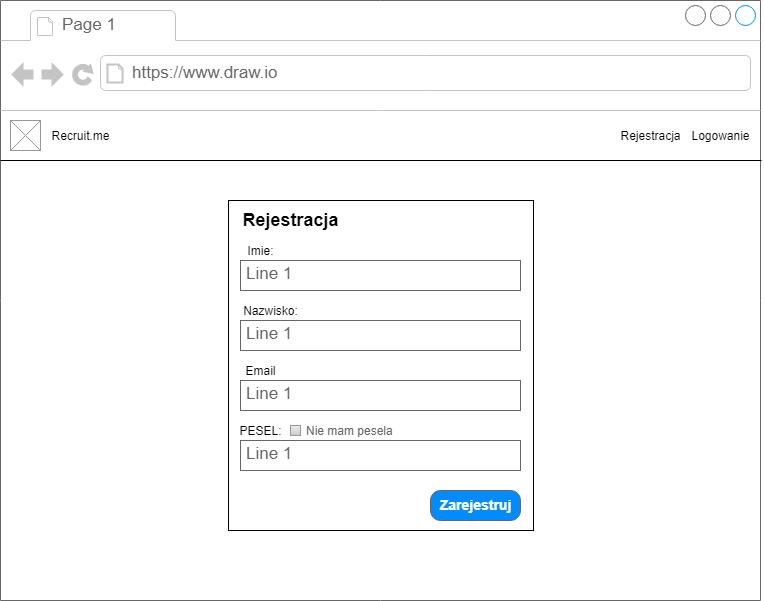
\includegraphics[width=\linewidth,height=\textheight,keepaspectratio=true]{images/rejestracjaMockup.png}
    \item Jako Kandydat mogę się zalogować, aby sprawdzić spersonalizowane informacje dotyczące rekrutacji.
        \begin{itemize}
            \item Logowanie odbywa się za pomocą ID kandydata oraz hasła.
            \item Aplikacja rozpoznaje czy obecny Użytkownik jest zalogowany.
            \item Część funkcjonalności jest dostępna tylko dla zalogowanych użytkowników.
        \end{itemize}
    \item Jako Kandydat mogę zresetować hasło, aby nie utracić dostępu do Systemu. 
        \begin{itemize}
            \item Na prośbę Systemu podaję otrzymany na koniec procesu rejestracji ID Kandydata i na podany w procesie rejestracji e-mail otrzymuję link do zmiany hasła.
        \end{itemize}
    \item Jako Kandydat mogę dostać przypomnienie ID Kandydata, aby nie utracić dostępu do Systemu. 
        \begin{itemize}
            \item Na prośbę Systemu podaję adres e-mail oraz numer PESEL (lub imię i nazwisko, gdy brak PESELu) podane w trakcie rejestracji. Jeśli wskazany e-mail znajduje się w Systemie i jest potwierdzony, zostaje na niego wysłana informacja o koncie Kandydata o podanym wcześniej adresie e-mail i danych potwierdzających (numer PESEL lub imię i nazwisko).
        \end{itemize}
    \item Jako zalogowany Kandydat otworzyć stronę swojego profilu, aby edytować swoje dane.   
        \begin{itemize}
            \item Strona wyświetla dane podane przy rejestracji, jednak są one zablokowane do edycji.
            \item Wyświetlane są pozostałe dane do edycji
                \begin{itemize}
                    \item Imiona i nazwiska rodziców
                    \item Nazwa szkoły podstawowej
                    \item Adres zamieszkania.
                \end{itemize}
            \item Strona profilu umożliwia przesłanie zdjęcia profilowego (patrz poniżej).
            \item Strona profilu umożliwia przesłanie dodatkowych dokumentów (maksymalnie 10, każde o rozmiarze maksymalnie 4MB).
        \end{itemize}
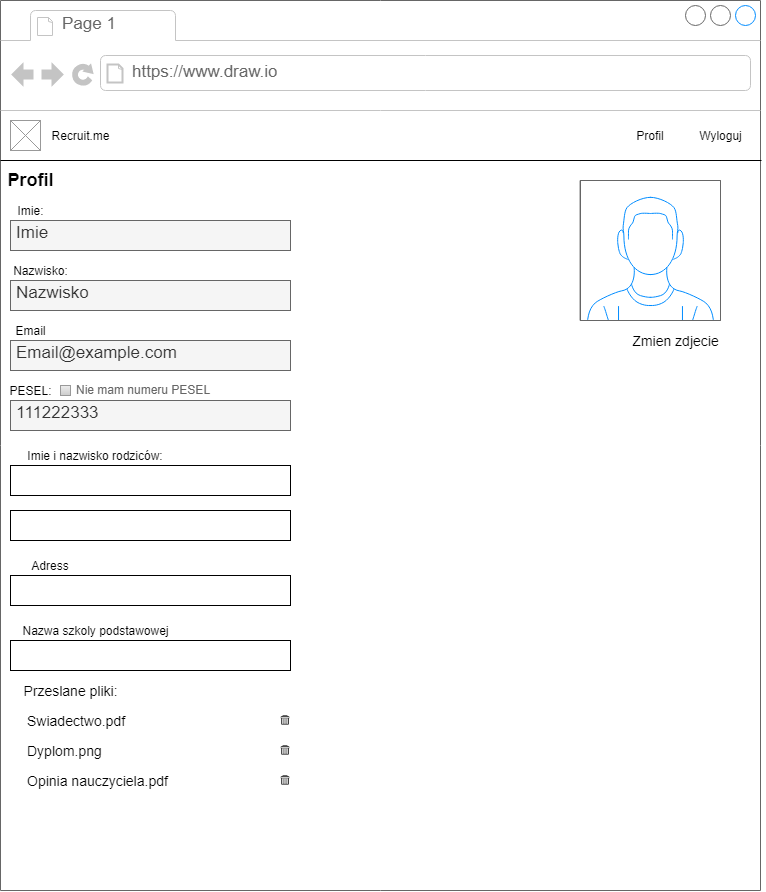
\includegraphics[width=\linewidth,height=\textheight,keepaspectratio=true]{images/profilMockup.png}
    \item Jako zalogowany kandydat mogę dodać zdjęcie profilowe, aby być rozpoznawanym w systemie.
        \begin{itemize}
        \item Zdjęcie mogę wprowadzić na dwa sposoby: wybierając już istniejący plik z dysku lub robiąc sobie zdjęcie kamerką w urządzeniu (jeżeli taka jest).
        \item Miniaturka zdjęcia pokazuje się na stronie profilu.
        \item Zdjęcie może być przeze mnie podmieniane na nowe.
        \end{itemize}
    \item Jako zalogowany Kandydat mogę dokonać opłaty za rejestrację, aby dokończyć rejestrację.
        \begin{itemize}
            \item Strona profilu wyświetla obecny stan transakcji (nieopłacona, w trakcie, opłacona).
            \item Transakcja odbywa się przez internetową bramkę płatniczą.
            \item Po potwierdzeniu płatności Kandydat jest automatycznie przypisany do Egzaminów.
        \end{itemize}
    \item Jako Kandydat, który dokonał płatności, mogę sprawdzić terminy swoich egzaminów, aby do nich przystąpić.
        \begin{itemize}
            \item Wyświetla się termin, miejsce, rodzaj egzaminu oraz typ.
        \end{itemize}
    \item Jako Kandydat, mogę zadać pytanie organizatorom poprzez stronę internetową, aby ułatwić komunikację ze Szkołą.
        \begin{itemize}
            \item Zadane pytania wyświetlają się w formie chatu.
            \item Kiedy jest otwarta dana zakładka, strona wiadomości synchronizują się co 15 sekund.
        \end{itemize}
    \item Jako Kandydat, mogę sprawdzić stan rekrutacji - przyjęty, nieprzyjęty, w trakcie.
        \begin{itemize}
            \item Aktualny stan rekrutacji będzie widoczny na stronie profilu
        \end{itemize}
\end{enumerate}

\subsection{Organizator Rejestracji}
\begin{enumerate}
  \item Jako Organizator mogę zalogować się do Aplikacji, aby nadzorować proces rekrutacji.
      \begin{itemize}
         \item Aplikacja rozpoznaje, że zalogowany Użytkownik jest Organizatorem.
         \item Funkcjonalności Organizatora różnią się od funkcjonalności Kandydata (patrz poniżej).
       \end{itemize}
  \item Jako Organizator mogę zarządzać danymi w Systemie, aby obsłużyć nieprzewidziane przypadki oraz sprawdzić wprowadzone informację.
      \begin{itemize}
         \item Stworzona zostanie strona Organizatora umożliwiająca odczyt, edycję i usuwanie obiektów w Systemie.
       \end{itemize}
  \item Jako Organizator mogę komunikować się z Kandydatami przez chat.
      \begin{itemize}
         \item Wylistowane są konwersacje z kandydatami, według daty ostatniej wiadomości.
         \item Po kliknięciu w daną konwersację mogę odczytać całą konwersację oraz wysłać nową wiadomość.
         \item Gdy tylko zostanie wysłana nowa wiadomość, na stronie profilu Kandydata będzie widoczne powiadomienie o nowej wiadomości.
       \end{itemize}
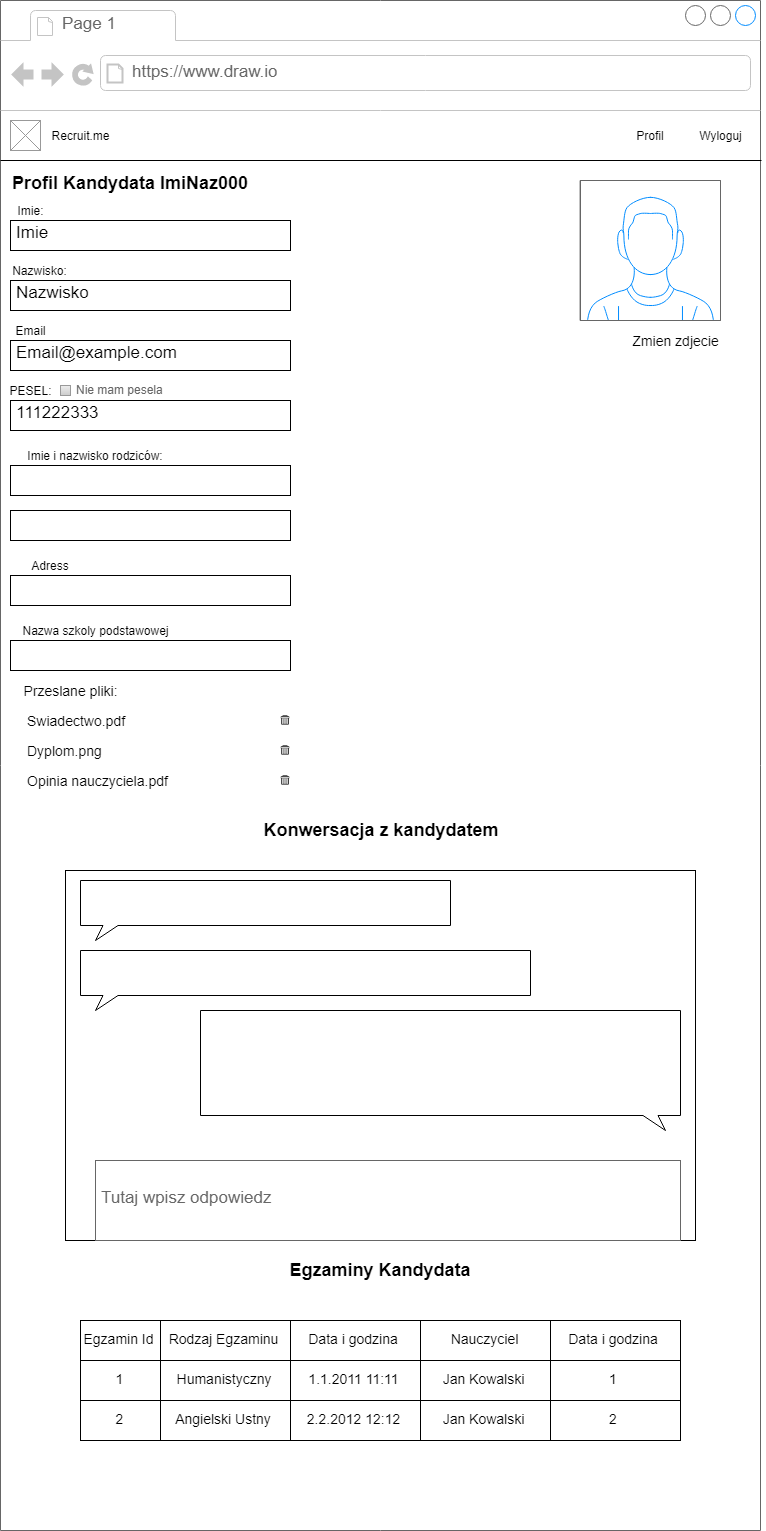
\includegraphics[height=\textheight,keepaspectratio=true]{images/AdminViewProfilKandydata.png}
  \item Jako Organizator mam dostęp do strony umożliwiającej zarządzanie egzaminami, aby usprawnić zarządzanie Rekrutacją.
      \begin{itemize}
         \item Aby utworzyć egzamin muszę podać: 
            \begin{itemize}
                \item Rodzaj Egzaminu
                \item Forma Egzaminu (wspólny, indywidualny)
                \item Miejsce, data i godzina rozpoczęcia
                \item Czas trwania
                \item Limit kandydatów.
            \end{itemize}
         \item Po dokonaniu opłaty Kandydatowi jest przypisywany po jednym Egzaminie z każdego rodzaju. Jeśli egzamin jest pisemny, godziną egzaminu jest godzina rozpoczęcia, jeśli egzamin jest ustny to jest to (godzina rozpoczęcia + czas trwania * [numer na liście - 1])
         \item Mogę edytować listę Kandydatów przystępujących do danego Egzaminu.
       \end{itemize}
  \item Jako Organizator mogę generować identyfikatory Kandydatów, aby łatwiej przeprowadzać egzaminy.
      \begin{itemize}
         \item Identyfikator jest generowany według pewnego szablonu i zawiera takie informacje jak: zdjęcie profilowe Kandydata, jego imię, nazwisko i ID, zakodowane dane kandydata, np.: w formie kodu QR, umożliwiające elektroniczne rozpoznanie Kandydata.
       \end{itemize}
  \item Jako Organizator mogę wprowadzać do systemu nauczycieli, którzy będą nadzorować proces egzaminowania.
      \begin{itemize}
         \item Nauczycielom NIE jest tworzone konto w systemie.
         \item Dane o nauczycielach są potrzebne przy wprowadzaniu ocen z egzaminów(patrz poniżej).
       \end{itemize}
\end{enumerate}

\subsection{Skanowanie kart ocen}
\begin{enumerate}
    \item Jako Organizator mogę wygenerować w Systemie dokumenty ułatwiające wprowadzanie ocen.
    \begin{itemize}
        \item Dokument zawiera dane takie jak: Id Nauczyciela, Id Kandydata, Id Egzaminu, ocenę z egzaminu
        \item Wygenerowany dokument jest według ściśle określonego szablonu i  jest dostosowany do przetwarzania OMR.
    \end{itemize}
  \item Jako Organizator mogę wprowadzić do Systemu wypełnione karty ocen, aby szybko wprowadzić dane do Systemu.
    \begin{itemize}
        \item Mogę wprowadzić wiele plików na raz.
        \item Odczytane dane: dane Nauczyciela, Kandydata i Egzaminu, będą wprowadzone automatycznie do Systemu.
   \end{itemize}
\end{enumerate}

\subsection{Drukowanie identyfikatorów}
\begin{enumerate}
    \item Jako Organizator mogę pobrać z Systemu plik z listą Kandydatów zawierającą ich zdjęcie, Identyfikator, imię, nazwisko oraz listę egzaminów, w jakich biorą udział
        
\end{enumerate}

\section{Wymagania niefunkcjonalne}

\begin{itemize}
	\item Komunikacja wewnątrz Systemu odbywa się poprzez protokół HTTPS.
	\item Wszystkie akcje użytkownika są autoryzowane na podstawie kryptograficznie podpisanego tokenu.
	\item Wywołanie każdej funkcjonalności jest poprzedzone sprawdzeniem czy obecny Użytkownik jest do niej uprawniony, w szczególności funkcjonalności Organizatora.
	\item Aplikacja będzie dostępna przez co najmniej dwadzieścia dwie godziny w ciągu doby w okresie rekrutacyjnym.
	\item Architektura zapewnia bezproblemowe równoległe korzystanie z systemu przez co najmniej stu użytkowników.
	\item Przy połączeniu szerokopasmowym, wywołany przez użytkownika interfejs otworzy się po czasie nie dłuższym niż trzy sekundy. 
	\item Aplikacja będzie działała bezproblemowo na:
	    \begin{itemize}
	        \item Przeglądarkach internetowych Google Chrome, Opera, Mozilla Firefox, Safari, Microsoft Edge oraz Internet Explorer od wersji odpowiednio 60, 50, 60, 10.1, 15 oraz 11
	        \item telefonach komórkowych z systemem Android od wersji 4.1.
	    \end{itemize}
	\item Aplikacja mobilna nie zadziała na telefonach, w których nie ma możliwości zainstalowania zewnętrznych aplikacji.
	\item Aplikacja webowa i mobilna do poprawnego działania wymaga połączenia z Internetem. Na urządzeniach bez możliwości połączenia z Internetem, aplikacja webowa i mobilna nie zadziałają.
\end{itemize}

Aplikacja mobilna do swojego działania wykorzystuje możliwości przez obecne urządzenia mobilne. Aby zapewnić poprawne działanie aplikacji mobilnej, przy instalacji aplikacji mobilnej lub przy pierwszym użyciu funkcji aplikacji korzystającego z danego modułu telefonu, użytkownik będzie proszony o zgodę na:
\begin{itemize}
	\item \textbf{odbieranie danych z internetu i pełny dostęp do sieci} – na potrzeby prawidłowej rejestracji, dokonania płatności i zapisania na egzamin,
	\item \textbf{wyświetlanie połączeń sieciowych} – na potrzeby sprawdzania dostępu do internetu przez aplikację,
	\item \textbf{dostęp do aparatu} - na potrzeby zrobienia zdjęcia do profilu kandydata
	\item \textbf{dostęp do multimediów} - na potrzeby wybrania zdjęcia do profilu kandydata
\end{itemize}

\section{Analiza SWOT}

Poniżej jest zamieszczona analiza ryzyka naszego projektu. 
\begin{itemize}
    \item \textbf{Mocne strony}
    \begin{itemize}
        \item Zespół ma doświadczenie w pisaniu aplikacji z interfejsem webowym, co znacznie przyspiesza proces tworzenia produktu
        \item Projekt jest łatwo rozszerzalny o nowe funkcjonalności, które mogą być dodane w zależności od oczekiwań 
        \item System nie wymaga dużej serwerowni do uruchomienia - pozwala na zainstalowanie systemu na dostępnych maszynach danej szkoły lub skorzystanie z rozwiązania chmurowego
    \end{itemize}
    
    \item \textbf{Słabe strony}
    \begin{itemize}
        \item Uzależnienie aplikacji od połączenia internetowego - awaria Internetu uniemożliwia praktycznie dostęp i korzystanie z systemu
        \item Powolny proces dostosowywania aplikacji do potrzeb odbiorcy, jeżeli te są bardzo wymagające 
    \end{itemize}
    
    \item \textbf{Szanse}
    \begin{itemize}
        \item Przejrzysta aplikacja mobilna szansą na zainteresowanie się projektem większej liczby instytucji
        \item Duża liczba istniejących już na rynku systemów rekrutacji
        \item Dobrze udokumentowane narzędzia do tworzenia aplikacji webowej i aplikacji mobilnej
    \end{itemize}
    
    \item \textbf{Zagrożenia}
    \begin{itemize}
        \item Silna pozycja na rynku istniejących systemów rekrutacji
        \item Ustalony termin ukończenia prac nad systemem może spowodować brak realizacji założonych wcześniej funkcjonalności
        \item Inne zobowiązania zespołu wobec uczelni mogą wpłynąć negatywnie na czas poświęcony na tworzenie aplikacji
    \end{itemize}
\end{itemize}

\section{Harmonogram}

Harmonogram przedstawia przewidywany plan działania dla projektu. Tabelka zawiera piętnaście, dwukolumnowych wierszy. W pierwszej kolumnie każdego wiersza poniższej tabelki znajdziemy numer tygodnia, który jest rozpatrywany. Druga kolumna natomiast zawiera listę zadań, które mają być wykonane w danym tygodniu.

\begin{center}
	\begin{tabular}{|c|L|}
	\hline
	Numer tygodnia & Lista zadań \\
	\hline
	Tydzień 1. & Analiza działania systemu, instalacja środowiska do implementacji projektu\\
	\hline
	Tydzień 2. & Stworzenie dokumentu analizy wymagań, implementacja autentykacji i autoryzacji, implementacja routingu aplikacji mobilnej\\
	\hline
	Tydzień 3. & Dopracowanie dokumentu analizy wymagań, testy manualne autentykacji i autoryzacji, pisanie pierwszych formularzy aplikacji mobilnej\\
	\hline
	Tydzień 4. & Akceptacja analizy wymagań przez promotora, opracowanie architektury systemu, uszczegółowienie listy wymaganych modułów \\
	\hline
	Tydzień 5. & Implementacja głównych modułów 1/3 \\
	\hline
	Tydzień 6. & Implementacja głównych modułów 2/3 \\
	\hline
	Tydzień 7. & Implementacja głównych modułów 3/3 \\
	\hline
	Tydzień 8. & Integracja głównych modułów 1/2, testy jednostkowe głównych modułów 1/2 \\
	\hline
	Tydzień 9. & Integracja głównych modułów 2/2, testy jednostkowe głównych modułów 1/2 \\
	\hline
	Tydzień 10. & Testy integracyjne 1/2, pisanie dokumentacji 1/4 (wstęp) \\
	\hline
	Tydzień 11. & Testy integracyjne 2/2, pisanie dokumentacji 2/4 (opis użytych technologii, funkcjonalności) \\
	\hline
	Tydzień 12. & Tworzenie opcjonalnych funkcjonalności 1/2, pisanie dokumentacji 3/4 (user guide, step-by-step deploy guide) \\
	\hline
	Tydzień 13. & Tworzenie opcjonalnych funkcjonalności 2/2, pisanie dokumentacji 4/4 (poprawki estetyczno-gramatyczne) \\
	\hline
	Tydzień 14. & Dopisanie ostatnich testów, przygotowanie makiet projektu \\
	\hline
	Tydzień 15. & Przerzucenie ostatecznej dokumentacji i wszystkich plików na płytę CD, oddanie projektu \\
	\hline
	\end{tabular}
\end{center}

\section{Lista zmian}

\begin{tabularx}{\linewidth}{|X|l|l|X|}
    \hline
    Autor & Data & Wersja & Wprowadzone zmiany \\
    \hline
    Filip Zyskowski & 28.10.2019 & v0.5 & Dodano analizę SWOT \\
    \hline
    Andrzej Westfalewicz & 24.10.2019 & v0.4 & Dodano ustalone wcześniej poprawki wymagań funkcjonalnych. Dodano makiety strony internetowej. \\
    \hline
    Andrzej Westfalewicz, Filip Zyskowski & 16.10.2019 & v0.3 & Dodano wymagania funkcjonalne, doprecyzowano słownik pojęć i wymagania niefunkcjonalne \\
    \hline
    Filip Zyskowski & 12.10.2019 & v0.2 & Dodany słownik pojęć \\
    \hline
    Filip Zyskowski & 11.10.2019 & v0.1 & Dodane wymagania niefunkcjonalne, harmonogram i opis systemu \\
    \hline
\end{tabularx}


\end{document}